\documentclass{article}

\usepackage[preprint]{neurips_2026}
\usepackage[utf8]{inputenc}
\usepackage[T1]{fontenc}
\usepackage{hyperref}
\usepackage{url}
\usepackage{booktabs}
\usepackage{amsfonts}
\usepackage{amsmath}
\usepackage{amssymb}
\usepackage{amsthm}
\usepackage{nicefrac}
\usepackage{microtype}
\usepackage{graphicx}
\usepackage{xcolor}
\usepackage{algorithm}
\usepackage{algorithmic}
\usepackage{subcaption}
\usepackage{thmtools}
\usepackage{thm-restate}

\newtheorem{proposition}{Proposition}
\newtheorem{corollary}{Corollary}
\newtheorem{remark}{Remark}
\theoremstyle{definition}
\newtheorem{definition}{Definition}

\title{Gradient Boosting within a Single Attention Layer\thanks{Code available at \url{https://github.com/salehsargolzaee/boosted-attention}}}

\author{
  Saleh Sargolzaei \\
  University of Windsor \\
  \texttt{sargolz@uwindsor.ca}
}

\begin{document}

\maketitle

\begin{abstract}
Transformer attention computes a single softmax-weighted average over values---a one-pass estimate that cannot correct its own errors.
We introduce \emph{gradient-boosted attention}, which applies the principle of gradient boosting \emph{within} a single attention layer: a second attention pass, with its own learned projections, attends to the prediction error of the first and applies a gated correction.
Under a squared reconstruction objective, the construction maps onto Friedman's gradient boosting machine, with each attention pass as a base learner and the per-dimension gate as the shrinkage parameter.
We show that a single Hopfield-style update erases all query information orthogonal to the stored-pattern subspace, and that further iteration under local contraction can collapse distinct queries in the same region to the same fixed point.
We also show that separate projections for the correction pass can recover residual information inaccessible to the shared-projection approach of Tukey's twicing.
On a 10M-token subset of WikiText-103, gradient-boosted attention achieves a test perplexity of $67.9$ compared to $72.2$ for standard attention, $69.6$ for Twicing Attention, and $69.0$ for a parameter-matched wider baseline, with two rounds capturing most of the benefit.
\end{abstract}


% ============================================================
\section{Introduction}
\label{sec:intro}
% ============================================================

The attention mechanism \citep{vaswani2017attention} computes a softmax-weighted combination of value vectors, conditioned on query-key similarities.
This is a single-pass operation: the query is compared against all keys once, a probability distribution is formed, and values are averaged accordingly.
If the resulting estimate is poor---because the query is ambiguous, the relevant keys are diluted among many distractors, or the softmax assigns weight to incompatible values---there is no within-layer mechanism to detect or correct the error.

A parallel limitation has long been understood in classical machine learning.
A single regression tree or a single kernel smoother produces a biased estimate; the bias can be reduced by fitting a second model to the \emph{residual} of the first.
This is the insight behind gradient boosting \citep{friedman2001greedy}, which builds an additive model $F = f_0 + \eta_1 f_1 + \eta_2 f_2 + \cdots$ by sequentially fitting each $f_m$ to the negative gradient of the loss with respect to the current prediction.
With strong base learners, two or three rounds often suffice \citep{friedman2001greedy}.

We apply this principle within a single attention layer.
Round~0 produces an initial estimate via standard attention.
The residual---the difference between the input and this estimate---is then passed through a second attention round with its own learned $\mathbf{W}_Q, \mathbf{W}_K, \mathbf{W}_V$ projections, where all three projections operate on the residual signal.
A per-dimension learned gate controls how much of the correction to apply.
Crucially, the second round derives its keys and values from the residual, allowing it to operate in a different subspace than the first round and recover information that shared-kernel corrections cannot amplify.
The result is a drop-in replacement for standard attention that adds one extra set of projections and a small gating network (approximately 18\% additional parameters overall).

\paragraph{Why not simply iterate attention?}
A natural alternative is to iterate the same attention operation: given output $\hat{y}$, feed it back as the query and repeat.
This corresponds to running the modern Hopfield network \citep{ramsauer2021hopfield} toward its fixed point.
We show (Section~\ref{sec:theory}, Proposition~\ref{prop:erasure}) that this approach systematically destroys query information.
Under the local contraction conditions established by \citet{ramsauer2021hopfield}, queries in the same contraction region converge to the same fixed point, which is determined by the stored patterns and temperature alone.
This makes iteration appropriate for content-addressable memory (where the goal is to retrieve a stored pattern) but harmful for the transformer's actual task (where the query carries information that must be preserved in the output).
Our negative results---including training with Deep Equilibrium Models \citep{bai2019deep}---confirm that the iterative approach failed under all training procedures we tested (Section~\ref{sec:negative}).
Gradient-boosted attention avoids this failure mode by feeding a \emph{different} signal (the residual) through \emph{different} projections, rather than re-processing the same state through the same function.

\paragraph{Relation to prior work.}
The idea that transformers implement a form of gradient descent is not new.
\citet{cheng2024transformers} proved that each transformer layer implements one step of functional gradient descent in a reproducing kernel Hilbert space---which is, mathematically, one round of gradient boosting---though they did not make this connection to the boosting literature explicit.
\citet{abdullaev2025twicing} applied Tukey's twicing \citep{tukey1977exploratory} within each attention layer, smoothing the residual $\mathbf{V} - \mathbf{A}\mathbf{V}$ with the \emph{same} attention matrix $\mathbf{A}$.
Their correction reuses the same attention kernel, yielding $(2\mathbf{A} - \mathbf{A}^2)\mathbf{V}$, without learned gating or separate projections for the correction pass.
Differential Transformer \citep{ye2025differential} computes two attention maps in parallel and subtracts them, canceling shared noise; this is a parallel subtractive mechanism, while ours is sequential and error-corrective.
We discuss these and other related works in detail in Section~\ref{sec:related}.

\paragraph{Contributions.}
\begin{enumerate}
    \item We introduce gradient-boosted attention, a multi-round attention mechanism in which each round corrects the prediction error of previous rounds using separate learned projections and a per-dimension gate. The architecture maps directly onto Friedman's MART framework.

    \item We show that a single attention step discards all query information orthogonal to the stored patterns (Proposition~\ref{prop:erasure}), establish a formal correspondence to Friedman's gradient boosting under a reconstruction objective (Proposition~\ref{prop:mart}), and show that separate projections applied to the residual can both attend to different tokens and produce values in a different subspace than the first round, escaping the convex hull of the original value vectors (Proposition~\ref{prop:separate}).

    \item On a 10M-token subset of WikiText-103, gradient-boosted attention improves test perplexity by $6.0\%$ relative over standard attention, outperforms Twicing Attention by $1.7$ points, and improves $1.1$ points over a parameter-matched wider baseline, with ablations confirming that two rounds capture most of the benefit.
\end{enumerate}


% ============================================================
\section{Background}
\label{sec:background}
% ============================================================

\subsection{Gradient Boosting}

Gradient boosting \citep{friedman2001greedy} constructs an additive model $F_M(x) = \sum_{m=0}^{M} \eta_m f_m(x)$ by sequential residual fitting.
Starting from an initial estimate $F_0(x) = f_0(x)$, each subsequent base learner $f_m$ is fit to the negative gradient of the loss:
\begin{equation}
\label{eq:boosting}
    r_m = -\frac{\partial L(y, F)}{\partial F}\bigg|_{F=F_{m-1}(x)}, \qquad f_m \approx r_m, \qquad F_m = F_{m-1} + \eta_m f_m,
\end{equation}
where $\eta_m \in (0, 1]$ is a shrinkage parameter that regularizes the update.
For the squared loss $L = \frac{1}{2}\|y - F\|^2$, the negative gradient is simply the residual $r_m = y - F_{m-1}(x)$.
A key empirical finding is that with strong base learners (e.g., deep trees), two to three rounds often capture most of the achievable improvement, with rapidly diminishing returns thereafter.

\subsection{Attention as Hopfield Retrieval}

\citet{ramsauer2021hopfield} showed that transformer attention is mathematically equivalent to one step of the modern continuous Hopfield network.
Given stored patterns $\mathbf{X} = [\mathbf{x}_1, \ldots, \mathbf{x}_N] \in \mathbb{R}^{d \times N}$ and a query $\boldsymbol{\xi} \in \mathbb{R}^d$, the update rule is:
\begin{equation}
\label{eq:hopfield}
    T(\boldsymbol{\xi}) = \mathbf{X} \, \mathrm{softmax}(\beta \mathbf{X}^\top \boldsymbol{\xi}),
\end{equation}
where $\beta > 0$ is the inverse temperature.
Setting $\beta = 1/\sqrt{d_k}$ and allowing separate key/value projections recovers standard attention.
The associated energy function is
\begin{equation}
\label{eq:energy}
    E(\boldsymbol{\xi}) = -\frac{1}{\beta}\log\sum_{i=1}^{N} \exp(\beta \, \mathbf{x}_i^\top \boldsymbol{\xi}) + \frac{1}{2}\|\boldsymbol{\xi}\|^2 + \text{const},
\end{equation}
whose gradient yields the update rule as $\boldsymbol{\xi}_{\text{new}} = -\nabla_{\boldsymbol{\xi}} E(\boldsymbol{\xi}) + \boldsymbol{\xi} = T(\boldsymbol{\xi})$.
Ramsauer et al.\ proved that under sufficient pattern separation relative to $\beta$, the iterates $T^t(\boldsymbol{\xi})$ converge exponentially to fixed points, and identified three types: global averages over all patterns, metastable states averaging over subsets, and near-single-pattern retrieval.


% ============================================================
\section{Method}
\label{sec:method}
% ============================================================

\subsection{Gradient-Boosted Attention}

\begin{figure}[t]
\centering
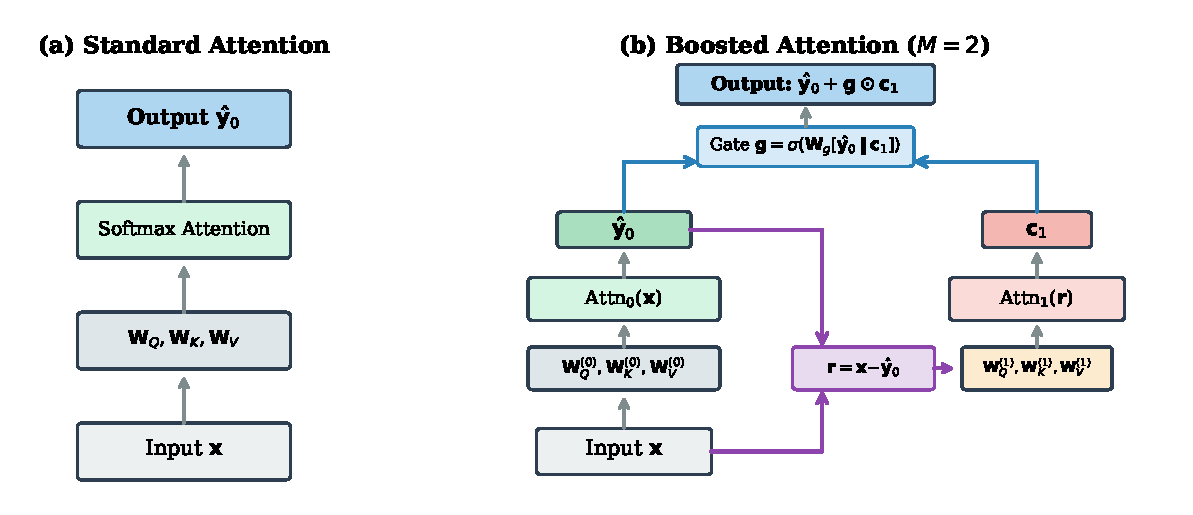
\includegraphics[width=\textwidth]{fig_architecture.pdf}
\caption{(a)~Standard attention computes a single softmax-weighted average. (b)~Gradient-boosted attention ($M{=}2$) adds a second pass where the prediction residual $\mathbf{r} = \mathbf{x} - \hat{\mathbf{y}}_0$ is projected through separate $\mathbf{W}_Q^{(1)}, \mathbf{W}_K^{(1)}, \mathbf{W}_V^{(1)}$ to produce queries, keys, and values. A learned gate $\mathbf{g}$ controls the per-dimension correction magnitude.}
\label{fig:architecture}
\end{figure}

Let $\mathbf{x} \in \mathbb{R}^{B \times T \times d}$ denote the input to an attention layer, and let $n_h$ denote the number of attention heads with per-head dimension $d_h = d / n_h$. We define $M$ attention rounds, each with its own learned projections $\mathbf{W}_Q^{(m)}, \mathbf{W}_K^{(m)}, \mathbf{W}_V^{(m)} \in \mathbb{R}^{d_h \times d}$ (per head):
\begin{equation}
\label{eq:attn_round}
    \mathrm{Attn}_m(\mathbf{z}) = \mathrm{softmax}\!\left(\frac{\mathbf{W}_Q^{(m)} \mathbf{z} \cdot (\mathbf{W}_K^{(m)} \mathbf{z})^\top}{\sqrt{d_h}}\right) \mathbf{W}_V^{(m)} \mathbf{z}.
\end{equation}
All three projections are applied to the same input $\mathbf{z}$: the original input $\mathbf{x}$ for round~0, and the current residual $\mathbf{r}_m$ for rounds $m \geq 1$.
Each correction round thus operates in its own subspace of the residual, with keys and values that reflect what has \emph{not yet been predicted} rather than the original context.

The forward pass (Algorithm~\ref{alg:boosted}) proceeds as follows:
\begin{algorithm}[t]
\caption{Gradient-Boosted Attention Forward Pass}
\label{alg:boosted}
\begin{algorithmic}[1]
\STATE \textbf{Input:} $\mathbf{x} \in \mathbb{R}^{B \times T \times d}$, number of rounds $M$
\STATE $\hat{\mathbf{y}}_0 \leftarrow \mathrm{Attn}_0(\mathbf{x})$ \hfill \COMMENT{Round 0: initial estimate}
\STATE $F \leftarrow \hat{\mathbf{y}}_0$
\FOR{$m = 1$ to $M-1$}
    \STATE $\mathbf{r}_m \leftarrow \mathbf{x} - F$ \hfill \COMMENT{Prediction error (negative gradient for $L_2$ loss)}
    \STATE $\mathbf{c}_m \leftarrow \mathrm{Attn}_m(\mathbf{r}_m)$ \hfill \COMMENT{Q, K, V all from residual via separate projections}
    \STATE $\mathbf{g}_m \leftarrow \sigma\!\left(\mathbf{W}_g^{(m)}[F \,\|\, \mathbf{c}_m]\right) \in [0,1]^d$ \hfill \COMMENT{Per-dimension shrinkage gate}
    \STATE $F \leftarrow F + \mathbf{g}_m \odot \mathbf{c}_m$ \hfill \COMMENT{Gated correction}
\ENDFOR
\STATE \textbf{Return:} $\mathbf{W}_{\mathrm{out}} \cdot F$
\end{algorithmic}
\end{algorithm}

\paragraph{The gate as a learned shrinkage parameter.}
In Friedman's framework, the shrinkage parameter $\eta_m$ is a scalar that regularizes each boosting step.
Our gate $\mathbf{g}_m = \sigma(\mathbf{W}_g^{(m)}[F \| \mathbf{c}_m]) \in [0,1]^d$ generalizes this in two ways: it is (i) per-dimension, allowing selective correction along different feature directions, and (ii) input-dependent, allowing the model to vary the correction magnitude based on the current prediction and the proposed correction.
When collapsed to a scalar, the gate reduces exactly to the shrinkage parameter.
We verify in our ablations (Section~\ref{sec:ablations}) that all gate variants (scalar, per-dimension, MLP) improve over the no-gate baseline, suggesting that the residual-attention mechanism is the primary ingredient.

\paragraph{Computational cost.}
With $M$ rounds, the attention computation is approximately $M$ times the cost of standard attention, plus a small gating network.
In practice, $M = 2$ adds approximately 18\% parameters and ${\sim}50\%$ attention FLOPs; however, since attention is only one component of each transformer block (alongside the FFN), the end-to-end wall-clock increase is approximately 20\% per training step.
By contrast, Twicing Attention \citep{abdullaev2025twicing} adds zero parameters and ${\sim}7\%$ total compute, since it reuses the same attention matrix.
Our additional cost buys separate projections for the correction pass, which Proposition~\ref{prop:separate} shows can recover information inaccessible to shared-kernel correction.
We show in Section~\ref{sec:experiments} that the improvement cannot be replicated by simply widening the standard model to match the parameter count.


\subsection{Connection to MART}
\label{sec:mart_connection}

Table~\ref{tab:mart} makes the correspondence between Friedman's Multiple Additive Regression Trees (MART) and gradient-boosted attention explicit.
Under the squared reconstruction objective $L = \frac{1}{2}\|\mathbf{x} - F\|^2$, the forward pass of Algorithm~\ref{alg:boosted} instantiates gradient boosting exactly: the residual is the negative gradient, each attention round is a base learner, and the gate is the shrinkage parameter.
Note that this is an internal objective governing the within-layer residual computation; the model is trained end-to-end with the task loss (e.g., cross-entropy for language modeling).

\begin{table}[t]
\centering
\caption{Correspondence between gradient boosting (MART) and gradient-boosted attention.}
\label{tab:mart}
\begin{tabular}{@{}lll@{}}
\toprule
\textbf{Component} & \textbf{MART} \citep{friedman2001greedy} & \textbf{Ours} \\
\midrule
Initial estimate & $f_0(x)$ (e.g., mean of targets) & $\hat{\mathbf{y}}_0 = \mathrm{Attn}_0(\mathbf{x})$ \\
Pseudo-residual & $r_m = y - F_{m-1}(x)$ & $\mathbf{r}_m = \mathbf{x} - F_{m-1}$ \\
Base learner & $f_m$ fit to $r_m$ & $\mathbf{c}_m = \mathrm{Attn}_m(\mathbf{r}_m)$ \\
Shrinkage & Scalar $\eta_m \in (0,1]$ & Gate $\mathbf{g}_m = \sigma(\mathbf{W}_g^{(m)}[\cdot]) \in [0,1]^d$ \\
Update & $F_m = F_{m-1} + \eta_m f_m$ & $F_m = F_{m-1} + \mathbf{g}_m \odot \mathbf{c}_m$ \\
\bottomrule
\end{tabular}
\end{table}


% ============================================================
\section{Theoretical Analysis}
\label{sec:theory}
% ============================================================

We present three results that collectively motivate and justify the gradient-boosted attention design.

\subsection{Iterating Attention Erases Query Information}

The most natural way to ``boost'' attention would be to iterate the same operation: compute $T(\boldsymbol{\xi})$, then $T(T(\boldsymbol{\xi}))$, and so on, converging to the Hopfield fixed point.
We show this approach is fundamentally flawed.

\begin{proposition}[One-step projection and information loss]
\label{prop:erasure}
Let $\mathbf{X} \in \mathbb{R}^{d \times N}$ be a matrix of stored patterns and $T(\boldsymbol{\xi}) = \mathbf{X}\,\mathrm{softmax}(\beta \mathbf{X}^\top \boldsymbol{\xi})$ the Hopfield update~(\ref{eq:hopfield}).
Then:
\begin{enumerate}
    \item[(a)] For every $\boldsymbol{\xi}$, $T(\boldsymbol{\xi}) \in \mathrm{conv}(\mathbf{X}) \subseteq \mathrm{col}(\mathbf{X})$.

    \item[(b)] If $\boldsymbol{\xi} = \boldsymbol{\xi}_\parallel + \boldsymbol{\xi}_\perp$ with $\boldsymbol{\xi}_\parallel \in \mathrm{col}(\mathbf{X})$ and $\boldsymbol{\xi}_\perp \perp \mathrm{col}(\mathbf{X})$, then $T(\boldsymbol{\xi}) = T(\boldsymbol{\xi}_\parallel)$.
    Hence all information in the component orthogonal to $\mathrm{col}(\mathbf{X})$ is erased after a single step.

    \item[(c)] Any fixed point $\boldsymbol{\xi}^*$ satisfies $\boldsymbol{\xi}^* = \mathbf{X}\,\mathrm{softmax}(\beta \mathbf{X}^\top \boldsymbol{\xi}^*)$, so every fixed point lies in $\mathrm{conv}(\mathbf{X})$.
\end{enumerate}
\end{proposition}

\begin{proof}
(a) Since $\mathrm{softmax}$ returns nonnegative weights summing to one, $T(\boldsymbol{\xi}) = \sum_{i=1}^N \alpha_i \mathbf{x}_i$ with $\alpha_i \geq 0, \sum_i \alpha_i = 1$, which is a convex combination of the columns of $\mathbf{X}$.

(b) The update $T(\boldsymbol{\xi})$ depends on $\boldsymbol{\xi}$ only through the score vector $\mathbf{X}^\top \boldsymbol{\xi}$.
Since $\mathbf{X}^\top \boldsymbol{\xi}_\perp = 0$ (each column of $\mathbf{X}$ is orthogonal to $\boldsymbol{\xi}_\perp$ by definition), we have $\mathbf{X}^\top \boldsymbol{\xi} = \mathbf{X}^\top \boldsymbol{\xi}_\parallel$, so $T(\boldsymbol{\xi}) = T(\boldsymbol{\xi}_\parallel)$.

(c) Setting $\boldsymbol{\xi} = \boldsymbol{\xi}^*$ in (a) gives $\boldsymbol{\xi}^* = T(\boldsymbol{\xi}^*) \in \mathrm{conv}(\mathbf{X})$. \qed
\end{proof}

\begin{remark}
\label{rem:erasure}
Proposition~\ref{prop:erasure} reveals a structural limitation of iterative Hopfield retrieval: after one step, the state is restricted to $\mathrm{conv}(\mathbf{X})$ and depends on the query only through the score vector $\mathbf{X}^\top \boldsymbol{\xi}$.
Any query information outside $\mathrm{col}(\mathbf{X})$ is immediately and irrecoverably discarded.
Further iteration compounds this: \citet{ramsauer2021hopfield} showed (their Lemma~A7) that under sufficient pattern separation, $T$ is a local contraction within a sphere around each stored pattern, with the Banach fixed-point theorem guaranteeing a unique fixed point per sphere.
Since these fixed points are determined by $\mathbf{X}$ and $\beta$ alone, distinct queries within the same local contraction region converge to the same output, erasing within-region query information.
This is consistent with the findings of \citet{smart2025incontext}, who showed that a single attention step can realize Bayes-optimal denoising behavior that outperforms both exact retrieval of a stored pattern and convergence to a potentially spurious local minimum.
Our experiments in Section~\ref{sec:negative} confirm this empirically: iterating trained attention to convergence degrades retrieval accuracy to near chance, while the one-step output retains useful query information.
\end{remark}


\subsection{Gradient-Boosted Attention as Gradient Boosting}

\begin{proposition}[MART equivalence]
\label{prop:mart}
Consider the squared prediction loss $L(\mathbf{x}, F) = \frac{1}{2}\|\mathbf{x} - F\|^2$, where $\mathbf{x}$ is the input and $F$ is the cumulative prediction from attention rounds $0, \ldots, m-1$.
Then the negative functional gradient of $L$ with respect to $F$ is
\begin{equation}
    -\nabla_F L(\mathbf{x}, F) = \mathbf{x} - F = \mathbf{r}_m,
\end{equation}
which is exactly the residual computed in line~5 of Algorithm~\ref{alg:boosted}.
Each correction round $\mathrm{Attn}_m(\mathbf{r}_m)$ fits a base learner (attention with separate projections) to this negative gradient, and the gated update $F_m = F_{m-1} + \mathbf{g}_m \odot \mathrm{Attn}_m(\mathbf{r}_m)$ is a shrinkage-regularized gradient boosting step.
\end{proposition}

\begin{proof}
The gradient is immediate from the loss definition.
The structural correspondence between Algorithm~\ref{alg:boosted} and the boosting update~(\ref{eq:boosting}) is exact when the loss is squared and the gate $\mathbf{g}_m$ plays the role of $\eta_m$.
The only difference is that $\eta_m$ in MART is a scalar optimized via line search, while $\mathbf{g}_m$ is a per-dimension function of the current state, learned jointly with the rest of the model by backpropagation. \qed
\end{proof}

\begin{remark}
\citet{cheng2024transformers} proved that the $L$-layer transformer implements $L$ steps of functional gradient descent in a reproducing kernel Hilbert space, but did not connect this to the classical boosting literature or to Friedman's MART.
Our construction makes this connection explicit and operates at a finer granularity: boosting within a single layer rather than across layers.
\end{remark}


\subsection{Why Separate Projections Are Necessary}

\citet{abdullaev2025twicing} proposed Twicing Attention, which smooths the residual $\mathbf{V} - \mathbf{A}\mathbf{V}$ using the \emph{same} attention matrix $\mathbf{A}$, yielding the output $(2\mathbf{A} - \mathbf{A}^2)\mathbf{V}$.
We show that reusing $\mathbf{A}$ imposes a key limitation.

\begin{proposition}[Limitation of shared attention in Twicing]
\label{prop:separate}
Let $\mathbf{A} = \mathrm{softmax}(\mathbf{Q}\mathbf{K}^\top / \sqrt{d_h})$ and consider the Twicing output
\begin{equation}
    (2\mathbf{A} - \mathbf{A}^2)\mathbf{V} = \mathbf{A}\mathbf{V} + \mathbf{A}(\mathbf{V} - \mathbf{A}\mathbf{V}).
\end{equation}
Both the base term and the correction term depend on the same attention weights $A_{ij}$ and the same value matrix $\mathbf{V}$.
In particular, if a token $j$ receives negligible attention weight ($A_{ij} \approx 0$ for all queries $i$), then its contribution to both $\mathbf{A}\mathbf{V}$ and $\mathbf{A}(\mathbf{V} - \mathbf{A}\mathbf{V})$ is negligible, regardless of the magnitude of its residual $\mathbf{V}_j - [\mathbf{A}\mathbf{V}]_j$.
Moreover, the correction output $(2\mathbf{A} - \mathbf{A}^2)\mathbf{V}$ remains in $\mathrm{conv}(\mathbf{V})$, the same convex hull as the base output $\mathbf{A}\mathbf{V}$.

In contrast, gradient-boosted attention computes the correction via $\mathrm{Attn}_1(\mathbf{r})$, where the residual $\mathbf{r} = \mathbf{x} - F_0$ is projected through separate $\mathbf{W}_Q^{(1)}, \mathbf{W}_K^{(1)}, \mathbf{W}_V^{(1)}$.
This differs from Twicing in two ways: (i) the attention matrix $\mathbf{A}' = \mathrm{softmax}(\mathbf{Q}'\mathbf{K}'^\top/\sqrt{d_h})$ is unconstrained by $\mathbf{A}$, so tokens that received negligible weight under $\mathbf{A}$ may receive significant weight under $\mathbf{A}'$; and (ii) the value vectors $\mathbf{V}' = \mathbf{W}_V^{(1)}\mathbf{r}$ span a different subspace than $\mathbf{V} = \mathbf{W}_V^{(0)}\mathbf{x}$, so the gated correction $F_0 + \mathbf{g} \odot \mathbf{A}'\mathbf{V}'$ can escape $\mathrm{conv}(\mathbf{V})$.
\end{proposition}

\begin{proof}
For Twicing, the correction term at position $i$ is
$[\mathbf{A}(\mathbf{V} - \mathbf{A}\mathbf{V})]_i = \sum_j A_{ij}(\mathbf{V}_j - [\mathbf{A}\mathbf{V}]_j)$.
The contribution of token $j$ is scaled by $A_{ij}$.
If $A_{ij} \approx 0$ for all $i$, then token $j$ contributes negligibly to both $\mathbf{A}\mathbf{V}$ and $\mathbf{A}(\mathbf{V}-\mathbf{A}\mathbf{V})$, regardless of the magnitude of its residual.
Furthermore, $(2\mathbf{A} - \mathbf{A}^2)\mathbf{V}$ where $2\mathbf{A} - \mathbf{A}^2$ is doubly stochastic (rows sum to one, entries are nonneg), so the output remains a convex combination of the rows of $\mathbf{V}$.

In gradient-boosted attention, the correction uses $\mathbf{A}'$ and $\mathbf{V}'$, both derived from $\mathbf{r}$ through separate projections.
Since $\mathbf{A}'$ is unconstrained by $\mathbf{A}$, it may attend to different tokens.
Since $\mathbf{V}' = \mathbf{W}_V^{(1)} \mathbf{r}$ and $\mathbf{V} = \mathbf{W}_V^{(0)} \mathbf{x}$ are produced by different projections of different inputs, $\mathrm{col}(\mathbf{V}')$ and $\mathrm{col}(\mathbf{V})$ are generically distinct, and $F_0 + \mathbf{g} \odot \mathbf{A}'\mathbf{V}'$ can lie outside $\mathrm{conv}(\mathbf{V})$. \qed
\end{proof}


% ============================================================
\section{Why Iterating Attention Fails: Negative Results}
\label{sec:negative}
% ============================================================

Before presenting our main experiments, we summarize the empirical evidence that motivated the gradient-boosted attention design.
These negative results complement Proposition~\ref{prop:erasure} by showing that the failure of iterative attention persists across the training methods and architectural modifications we tested.

We trained attention models on a pattern denoising task following the setup of \citet{smart2025incontext}: $K$ normalized patterns in $\mathbb{R}^d$, queries corrupted by additive Gaussian noise with standard deviation $\sigma$, evaluated by nearest-pattern retrieval accuracy.
Table~\ref{tab:negative} summarizes results across six configurations.

\begin{table}[t]
\centering
\caption{Retrieval accuracy (\%) for one-step attention vs.\ DEQ-trained converged attention. Random chance is $100/K$. Across all configurations, convergence degrades accuracy to near chance. Learned routing gates (5 feature sets) never exceed one-step accuracy.}
\label{tab:negative}
\begin{tabular}{@{}lcccccc@{}}
\toprule
& \multicolumn{2}{c}{$d{=}16, K{=}4$} & \multicolumn{2}{c}{$d{=}32, K{=}8$} & \multicolumn{2}{c}{$d{=}64, K{=}16$} \\
\cmidrule(lr){2-3} \cmidrule(lr){4-5} \cmidrule(lr){6-7}
& $\sigma{=}0.5$ & $\sigma{=}0.8$ & $\sigma{=}0.5$ & $\sigma{=}0.8$ & $\sigma{=}0.5$ & $\sigma{=}0.8$ \\
\midrule
Random chance & 25.0 & 25.0 & 12.5 & 12.5 & 6.3 & 6.3 \\
One-step (trained) & 78.9 & 59.7 & 59.8 & 39.5 & 39.2 & 22.9 \\
DEQ converged (trained) & 25.6 & 25.6 & 11.9 & 11.9 & 5.6 & 5.6 \\
\bottomrule
\end{tabular}
\end{table}

\paragraph{Iterating attention destroys accuracy.}
Across all six configurations in Table~\ref{tab:negative}, the DEQ-trained converged path achieves accuracy indistinguishable from random chance (e.g., 5.6\% vs.\ 6.3\% chance for $K{=}16$), while one-step attention achieves 22--79\% depending on the difficulty.
This is consistent with Proposition~\ref{prop:erasure} and the local-contraction analysis of \citet{ramsauer2021hopfield}: queries in the same contraction region converge to the same fixed point regardless of their initial position.

\paragraph{Implicit differentiation does not help.}
One might suspect the failure is due to vanishing gradients through many iteration steps.
We used Deep Equilibrium Models \citep{bai2019deep} to provide exact gradients at the fixed point via the implicit function theorem, bypassing the iterative computation graph entirely.
The converged path still achieved random-chance accuracy (Table~\ref{tab:negative}), confirming that the information loss is structural---a consequence of the contraction dynamics---not a training artifact.

\paragraph{Learned routing gates learn trivial strategies.}
We trained routing gates with five different feature sets (both outputs, their difference, scalar divergence, attention entropy) to decide when to trust the converged path.
All gates learned to always select the one-step output, achieving identical accuracy to the one-step baseline.
The converged path contains no useful complementary signal.


% ============================================================
\section{Experiments}
\label{sec:experiments}
% ============================================================

\subsection{WikiText-103 Language Modeling}

\paragraph{Setup.}
We train small transformer language models from scratch on a \textbf{10M-token subset} of WikiText-103 \citep{merity2016pointer} (the full corpus contains ${\sim}103$M tokens) and compare four configurations: (1)~\textbf{Standard} causal multi-head attention with $d = 256$, 4 layers, and 4 heads (7.4M parameters); (2)~\textbf{Twicing} Attention \citep{abdullaev2025twicing} with the same architecture, applying the correction $(2\mathbf{A} - \mathbf{A}^2)\mathbf{V}$ at no additional parameter cost (7.4M parameters); (3)~a \textbf{parameter-fair} standard model with $d = 288$, matching the parameter count of the boosted model (8.8M parameters); and (4)~\textbf{gradient-boosted attention} ($M = 2$) with separate QKV projections per round and a per-dimension sigmoid gate (8.7M parameters).

All models use BPE tokenization (16K vocabulary), sequence length 256, AdamW optimizer with learning rate $3 \times 10^{-4}$, cosine schedule with 1500 warmup steps, weight tying, and gradient clipping at 1.0.
We train for 15 epochs over the 10M-token training subset and evaluate on the full WikiText-103 test set, reporting perplexity averaged over 2 random seeds.
All models are trained on a single NVIDIA RTX 2000 Ada (16GB); each run takes approximately 30 minutes.
Full hyperparameters are listed in Appendix~\ref{app:hyperparams}.

\paragraph{Results.}

\begin{table}[t]
\centering
\caption{WikiText-103 test perplexity (lower is better). Boosted-2 outperforms both the standard baseline and a wider standard model with matched parameter count, confirming the improvement is architectural.}
\label{tab:wikitext}
\begin{tabular}{@{}lccc@{}}
\toprule
\textbf{Model} & \textbf{Test PPL} & \textbf{Val PPL} & \textbf{Parameters} \\
\midrule
Standard ($d{=}256$)              & $72.2 \pm 0.3$ & $72.2 \pm 0.4$ & 7,419,392 \\
Twicing ($d{=}256$)               & $69.6 \pm 0.1$ & $70.3 \pm 0.0$ & 7,419,392 \\
Standard ($d{=}288$, param-fair)  & $69.0 \pm 0.1$ & $69.6 \pm 0.1$ & 8,789,184 \\
Gradient-boosted ($d{=}256$, $M{=}2$) & $\mathbf{67.9 \pm 0.1}$ & $\mathbf{68.1 \pm 0.2}$ & 8,734,208 \\
\bottomrule
\end{tabular}
\end{table}

Table~\ref{tab:wikitext} shows the results.
Gradient-boosted attention achieves a test perplexity of $67.9$, improving over standard attention by $4.3$ points ($6.0\%$ relative).
Three comparisons isolate different contributions.
Compared with Twicing ($69.6 \to 67.9$, $-1.7$ points), both methods correct the initial attention estimate, but separate projections with a learned gate outperform the fixed shared-kernel correction $(2\mathbf{A} - \mathbf{A}^2)\mathbf{V}$, validating Proposition~\ref{prop:separate}.
Compared with the parameter-matched wider baseline ($69.0 \to 67.9$, $-1.1$ points), the wider standard model has slightly more parameters ($8.8$M vs $8.7$M) yet lacks the error-correction mechanism; this gap isolates the architectural contribution of residual fitting.
The total improvement over standard attention ($72.2 \to 67.9$, $-4.3$ points, $6.0\%$ relative) combines both the architectural and capacity effects.

Standard deviations are tight ($\leq 0.3$) across all configurations, confirming that the results are stable across random seeds.

\begin{figure}[t]
\centering
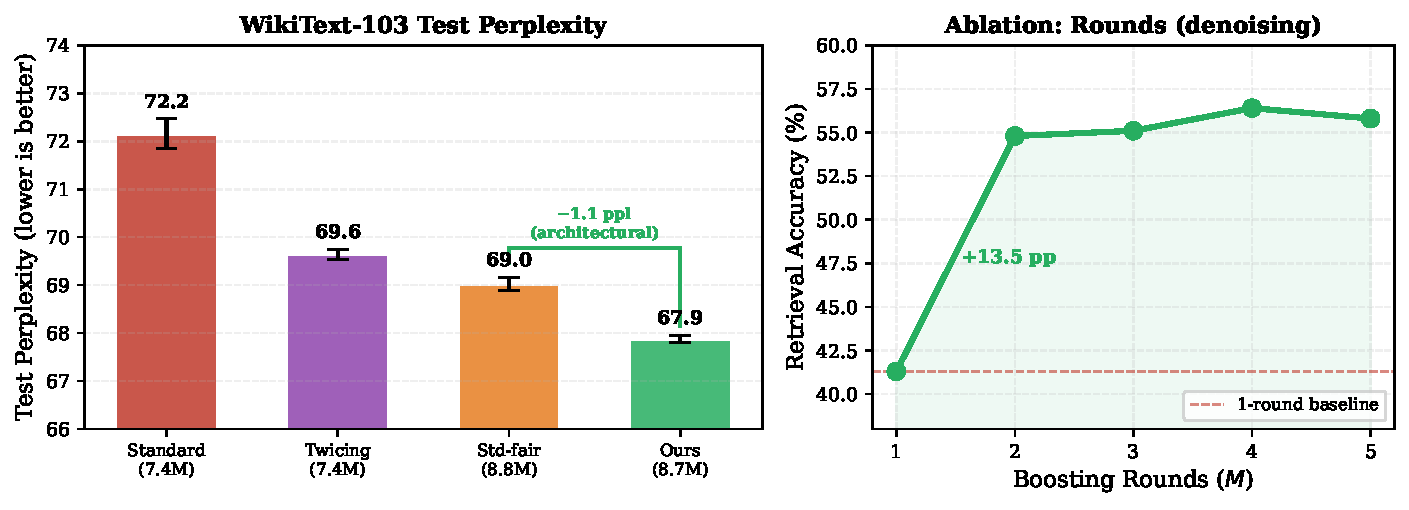
\includegraphics[width=\textwidth]{fig_results.pdf}
\caption{\textbf{Left:} WikiText-103 test perplexity (zoomed axis). Gradient-boosted attention outperforms all baselines including Twicing and a parameter-matched wider model. \textbf{Right:} Retrieval accuracy on the synthetic denoising task as a function of boosting rounds. The jump from 1 to 2 rounds captures most of the improvement.}
\label{fig:results}
\end{figure}


\subsection{Ablation Studies}
\label{sec:ablations}

We conduct ablations on the synthetic pattern denoising task ($d = 64$, $K = 16$ patterns, noise $\sigma = 0.5$) where the mechanism is most transparent.

\paragraph{Number of boosting rounds.}
Table~\ref{tab:rounds} shows retrieval accuracy as a function of $M$.
The jump from 1 to 2 rounds ($+12$ percentage points) accounts for the vast majority of the improvement.
Additional rounds provide diminishing returns: $+2$ for round 3, $+1$ for round 4.
This mirrors the well-known behavior of gradient boosting with strong base learners \citep{friedman2001greedy}, where early rounds capture the dominant signal and later rounds offer marginal gains.

\begin{table}[t]
\centering
\caption{Effect of boosting rounds on pattern retrieval accuracy (\%). Synthetic denoising task, $d=64$, $K=16$, $\sigma=0.5$.}
\label{tab:rounds}
\begin{tabular}{@{}lccccc@{}}
\toprule
\textbf{Rounds ($M$)} & 1 & 2 & 3 & 4 & 5 \\
\midrule
Accuracy (\%) & 41.3 & 53.3 & 54.8 & 56.3 & 55.8 \\
$\Delta$ from $M{=}1$ & --- & +12.0 & +13.5 & +15.0 & +14.5 \\
\bottomrule
\end{tabular}
\end{table}

\paragraph{Gate type.}
We compare three gate configurations with $M{=}2$ rounds: no gate ($\mathbf{g} = \mathbf{1}$, pure additive correction), scalar gate (one learned shrinkage value per round, matching the MART $\eta_m$), and per-dimension MLP gate.
All three produce similar accuracy: MLP gate 55.2\%, scalar gate 55.0\%, and no gate 54.3\%.
That even the no-gate variant performs comparably confirms that the residual-attention mechanism---not the gating---is the key ingredient.

\paragraph{Scaling with problem difficulty.}
The benefit of boosting grows with problem difficulty.
At $d = 64, K = 16, \sigma = 0.3$, the improvement is $+18.7$ percentage points.
At $d = 128, K = 32, \sigma = 0.3$, it is $+15.7$ points.
The correction helps most when the initial attention pass makes systematic but correctable errors---precisely the regime where gradient boosting is most effective.


\subsection{Analysis}
\label{sec:analysis}

We analyze the trained gradient-boosted models to understand what the correction round learns and where it helps most.

\paragraph{Gate values across layers.}
Figure~\ref{fig:gate_analysis} shows the learned per-dimension gate values, averaged over test sequences, for each of the four transformer layers.
Layer~0 is the most conservative (mean gate value $0.33$, standard deviation $0.08$), admitting only a modest fraction of the correction.
Layer~1 uses the correction most aggressively (mean $0.49$) and exhibits the highest variance across dimensions ($\sigma = 0.22$), indicating that some dimensions rely heavily on the correction while others suppress it.
Layers~2 and~3 fall in between ($0.39$ and $0.36$, respectively).
The per-dimension variation across all layers confirms that the gate is performing non-trivial, dimension-specific shrinkage rather than acting as a uniform scalar---consistent with the per-dimension generalization of the MART shrinkage parameter $\eta_m$ described in Section~\ref{sec:mart_connection}.

\begin{figure}[t]
\centering
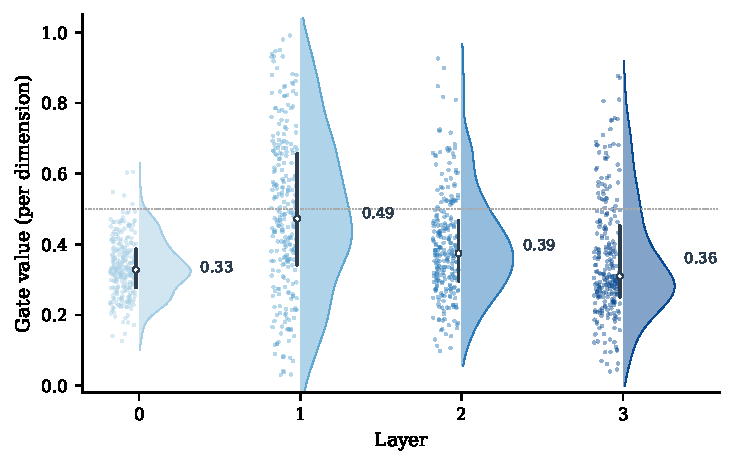
\includegraphics[width=0.7\textwidth]{fig_gate_analysis.pdf}
\caption{Learned gate values per dimension for each transformer layer, averaged over 50 test sequences. The dashed line marks $g = 0.5$. Gate magnitudes and variation differ across layers, with layer~1 applying the strongest and most selective correction.}
\label{fig:gate_analysis}
\end{figure}

\paragraph{Convex hull escape.}
Proposition~\ref{prop:erasure}(a) establishes that a single attention step maps every query into $\mathrm{conv}(\mathbf{V}^{(0)})$, the convex hull of the round-0 value vectors, since the softmax produces nonnegative weights summing to one.
Proposition~\ref{prop:separate} predicts that the gated correction can move the output \emph{outside} this hull, because the correction values $\mathbf{V}^{(1)} = \mathbf{W}_V^{(1)}\mathbf{r} \in \mathbb{R}^{T \times d_h}$ span a different subspace than $\mathbf{V}^{(0)} = \mathbf{W}_V^{(0)}\mathbf{x} \in \mathbb{R}^{T \times d_h}$.
We verify this quantitatively: for each attention head at a given position $t$, we compute the $\ell_2$ distance in $\mathbb{R}^{d_h}$ from the boosted output to the nearest point in $\mathrm{conv}(\mathbf{v}_1^{(0)}, \ldots, \mathbf{v}_t^{(0)})$---the convex hull of the causally visible round-0 value vectors for that head---by solving a convex quadratic program over the probability simplex (details in Appendix~\ref{app:convex_hull}).
A distance of zero means the output can be expressed as a convex combination of the round-0 values; any positive distance indicates escape.

Figure~\ref{fig:convex_hull} shows the distribution of these distances across 600 randomly sampled (position, head) pairs per layer.
Every measured output lies strictly outside $\mathrm{conv}(\mathbf{V}^{(0)})$ across all four layers (100\% escape rate).
The per-layer ranking mirrors the gate analysis: layer~1, which applies the strongest correction (mean gate~$0.49$), escapes farthest (mean $\ell_2$ distance~$5.19$), while layer~0, the most conservative (mean gate~$0.33$), stays closest (mean distance~$0.88$).
Layers~2 and~3 fall in between ($4.25$ and $3.41$, respectively).
This confirms that the correction round's separate projections produce representations outside the original value space, as predicted by Proposition~\ref{prop:separate}.

\begin{figure}[t]
\centering
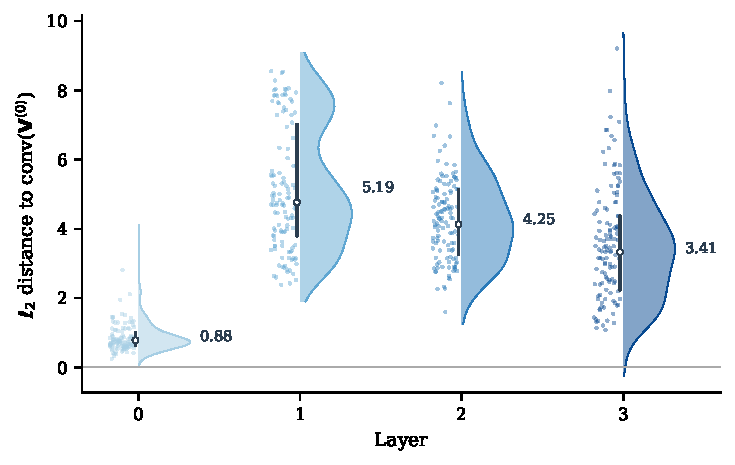
\includegraphics[width=0.7\textwidth]{fig_convex_hull.pdf}
\caption{$\ell_2$ distance in $\mathbb{R}^{d_h}$ ($d_h{=}64$) from the boosted output to the convex hull of round-0 value vectors $\mathrm{conv}(\mathbf{v}_1^{(0)}, \ldots, \mathbf{v}_t^{(0)})$, measured per attention head per position. Zero indicates the output lies within the hull; all 2{,}400 measured outputs are strictly positive, confirming escape at every layer. Annotated values are per-layer means. The ranking mirrors gate magnitudes (Figure~\ref{fig:gate_analysis}).}
\label{fig:convex_hull}
\end{figure}

\paragraph{Attention entropy.}
Figure~\ref{fig:attention_entropy} compares the entropy of the attention distributions between round~0 and round~1.
Across all layers and heads, the correction round exhibits 22\% lower entropy on average (3.31 vs.\ 2.58 nats), indicating that it attends more selectively than the initial round.
The per-layer breakdown reveals depth-dependent behavior: in layer~0, the correction round actually has slightly \emph{higher} entropy than the initial round, consistent with its conservative gate (mean $0.33$) allowing only a small fraction of a broadly-spread correction through.
In layers~1 and~2, the correction round is sharply focused (entropy drops by 55\% and 39\%, respectively), and these are also the layers where the gate admits the most correction (means $0.49$ and $0.39$).
This correlation between attention sharpness and gate openness suggests that the model learns to rely on the correction most when it can be made precise.

\begin{figure}[t]
\centering
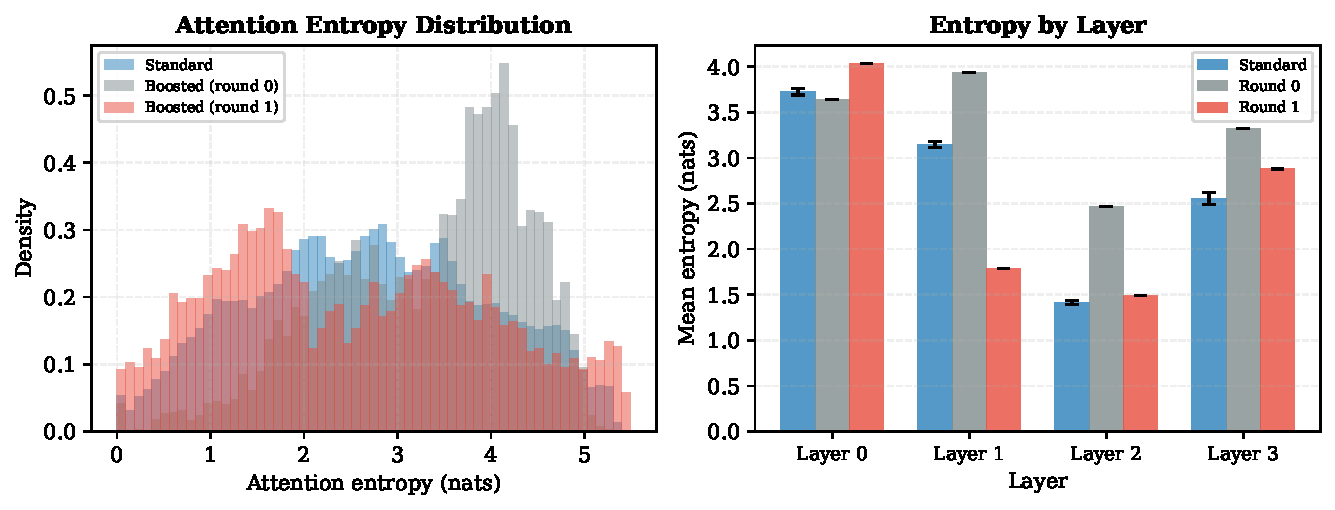
\includegraphics[width=\textwidth]{fig_attention_entropy.pdf}
\caption{\textbf{Left:} Distribution of attention entropy across all layers and heads for round~0 (initial) and round~1 (correction). The correction round is 22\% lower-entropy on average. \textbf{Right:} Mean entropy per layer. Layers~1--2 show the sharpest correction attention, coinciding with higher gate values (Figure~\ref{fig:gate_analysis}).}
\label{fig:attention_entropy}
\end{figure}

\paragraph{Example-level corrections.}
The aggregate statistics above show that the correction round attends more sharply; Figure~\ref{fig:examples} illustrates this on individual predictions.
We select three tokens (from different articles) where the boosted model dramatically outperforms standard attention, and overlay the head-averaged attention weights for round~0 and round~1 in layer~1.
In each case, round~0 distributes attention relatively uniformly across context tokens, while round~1 concentrates on the tokens most relevant to the target.
For instance, when predicting the continuation of ``Ke'' (target: ``iser,'' completing the name Keiser), round~1 places its highest weight on the preceding token ``Ke'' and the nearby geographical context, while standard attention predicts ``ong'' (confused by the earlier substring ``Yongsan'').
Similarly, for ``iron @-@ h'' $\to$ ``ul'' (completing ``hull''), round~1 attends sharply to ``iron,'' the hyphen, and ``h''---the compound being constructed---while standard attention predicts the wrong subword.
These examples are selected from the top of the per-token improvement distribution (improvement $>4.8$ nats) and thus illustrate the best-case rather than the typical behavior; the overall improvement of $4.3$ perplexity points reflects the average across all tokens.

\begin{figure}[t]
\centering
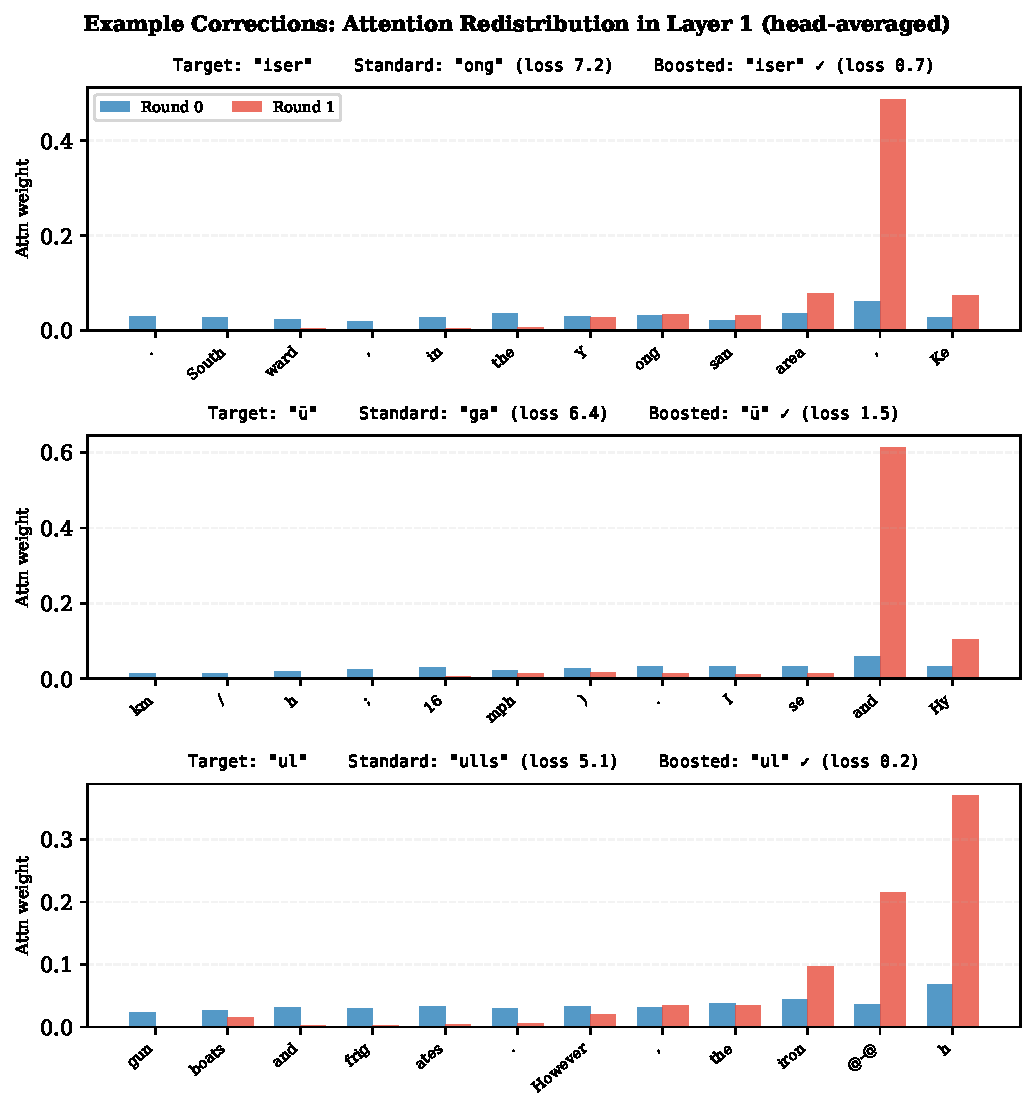
\includegraphics[width=0.85\textwidth]{fig_example_corrections.pdf}
\caption{Three tokens where gradient-boosted attention corrects a prediction error. Blue bars show round~0 attention (initial, diffuse); red bars show round~1 attention (correction, concentrated on relevant context). Each title shows the target token, the standard model's prediction, and the boosted model's prediction with cross-entropy loss. Layer~1, head-averaged.}
\label{fig:examples}
\end{figure}


% ============================================================
\section{Related Work}
\label{sec:related}
% ============================================================

\paragraph{Attention and Hopfield networks.}
\citet{ramsauer2021hopfield} established the equivalence between transformer attention and one step of the modern continuous Hopfield network, identifying three types of fixed points (global average, metastable states, single-pattern retrieval).
\citet{smart2025incontext} showed that a single trained attention step implements a gradient descent update on a context-aware dense associative memory energy landscape, and that this one-step estimate can be closer to the Bayes-optimal denoiser than the converged fixed point.
Our work extends these findings by proving why convergence fails (Proposition~\ref{prop:erasure}) and proposing a constructive alternative (gradient-boosted attention).

\paragraph{Transformers as gradient descent.}
\citet{cheng2024transformers} proved that each transformer layer implements one step of functional gradient descent in the RKHS associated with the attention kernel.
This result strengthens the view that transformers can implement stagewise functional optimization closely related to boosting, though Cheng et al.\ did not make this connection to the boosting literature explicit.
\citet{huang2018learning} showed that ResNet blocks can be interpreted as boosting stages, and \citet{siu2019residual} formalized this analogy.
\citet{badirli2020grownet} used shallow neural networks as base learners in a gradient boosting ensemble.
Our work differs from all of the above by applying boosting within a single attention operation, at a finer granularity than the layer level.

\paragraph{Residual correction in attention.}
The closest prior work is Twicing Attention \citep{abdullaev2025twicing}, which applies Tukey's twicing \citep{tukey1977exploratory} within each attention layer.
Their correction smooths the residual $\mathbf{V} - \mathbf{A}\mathbf{V}$ with the \emph{same} attention matrix $\mathbf{A}$, yielding $(2\mathbf{A} - \mathbf{A}^2)\mathbf{V}$.
The theoretical justification is from nonparametric statistics: twicing reduces the bias of the Nadaraya-Watson estimator \citep{newey2004twicing}.
Our approach differs in three ways: (i) we apply separate learned projections to the \emph{residual}, producing new queries, keys, \emph{and} values that can span a different subspace than the original attention (Proposition~\ref{prop:separate}); (ii) we include a learned gate that adapts the correction magnitude per-input and per-dimension; (iii) our framing as gradient boosting provides a different theoretical lens and suggests natural extensions (more rounds, adaptive halting).
A natural question is whether the fixed correction $(2\mathbf{A} - \mathbf{A}^2)\mathbf{V}$ is optimal, or whether learning separate projections for the correction pass can do better; our experiments in Section~\ref{sec:experiments} address this directly.

\paragraph{Attention variants.}
Differential Transformer \citep{ye2025differential} computes two parallel attention maps and takes their difference, canceling common-mode noise.
This is a parallel subtractive mechanism, orthogonal to our sequential error-corrective one; the two could in principle be combined.
Gated Attention \citep{qiu2025gated} adds a post-attention sigmoid gate per head, introducing non-linearity and sparsity into a single attention pass; it does not compute a second pass or attend to residuals.

\paragraph{Iterative computation in transformers.}
Universal Transformers \citep{dehghani2019universal} iterate the same transformer block with shared parameters and adaptive halting.
Deep Equilibrium Models \citep{bai2019deep} find the fixed point of a single layer via implicit differentiation.
PonderNet \citep{banino2021pondernet} learns when to stop iterating.
All iterate the \emph{same} function on the accumulated state.
Gradient-boosted attention differs by operating on the \emph{residual} with \emph{different} projections---a distinction that Proposition~\ref{prop:erasure} shows is critical.

\paragraph{Cross-layer residual methods.}
Several recent works improve information flow across transformer depth: DeepCrossAttention \citep{heddes2025deepcrossattention} replaces residual connections with depth-wise cross-attention, and Attention Residuals \citep{kimi2026attnres} replaces fixed skip connections with learned softmax attention over all preceding layer outputs, deployed at 48B-parameter scale.
These methods operate across layers; our approach operates within a single attention computation.


% ============================================================
\section{Discussion}
\label{sec:discussion}
% ============================================================

\paragraph{Limitations.}
Our experiments use small models (7--9M parameters) trained on a single benchmark with a limited number of tokens.
While the param-fair comparison controls for capacity, we have not yet established whether the improvement persists at the 100M--1B scale where most modern attention variants are evaluated \citep{ye2025differential}.
The additional computational cost of two attention passes per layer may be a concern for latency-sensitive applications, though the key-value computations could be shared to reduce overhead.

\paragraph{What scaling would show.}
The central question for future work is whether the 1.6\% relative improvement over a parameter-matched baseline holds, grows, or shrinks at larger model and data scales.
Gradient boosting typically helps most when individual learners are moderately strong---too weak and the residual is too noisy to fit, too strong and a single learner already captures most of the signal.
Attention in small models may be in the ``moderately strong'' regime where boosting is maximally effective; whether this persists at scale is an empirical question.

\paragraph{Future work.}
Natural extensions include: (i) applying gradient-boosted attention as a drop-in replacement during fine-tuning of pretrained models, which requires no large-scale pretraining; (ii) combining with Differential Transformer for joint noise cancellation and error correction; (iii) learning the number of rounds per head or per layer, analogous to adaptive boosting; (iv) analyzing whether the correction round develops interpretable specialization across heads and layers.

\paragraph{Broader motivation.}
Our architecture was partly motivated by the contrast between single-pass attention (a fast, parallel retrieval) and iterative convergence (a slower, sequential commitment to a single pattern)---a distinction reminiscent of dual-process theories in cognitive science.
The formal contribution, however, is the connection to gradient boosting, which provides precise theoretical tools rather than informal analogy.


% ============================================================
\section{Conclusion}
\label{sec:conclusion}
% ============================================================

We have introduced gradient-boosted attention, a mechanism that applies gradient boosting within a single attention layer.
A second attention pass, with its own learned projections, attends to the prediction error of the first pass and applies a gated correction.
We showed that the natural alternative---iterating the same attention operation---erases all query information orthogonal to the stored-pattern subspace, and under local contraction can collapse distinct queries in the same region to the same fixed point.
The formal correspondence to Friedman's MART framework connects a growing body of theoretical work on transformers-as-gradient-descent to the classical boosting literature.
Experiments on WikiText-103 confirm that gradient-boosted attention outperforms standard attention, Twicing Attention (which reuses the same attention kernel), and a parameter-matched wider baseline, with the improvement attributable to the architectural inductive bias of residual correction with separate projections.

\bibliography{references}
\bibliographystyle{plainnat}

\newpage
\appendix

\section{Hyperparameters and Training Details}
\label{app:hyperparams}

Table~\ref{tab:hyperparams} lists all hyperparameters for the WikiText-103 language modeling experiments.
All models share the same training configuration; only the attention mechanism differs.

\begin{table}[h]
\centering
\caption{Hyperparameters for WikiText-103 experiments.}
\label{tab:hyperparams}
\begin{tabular}{@{}ll@{}}
\toprule
\textbf{Hyperparameter} & \textbf{Value} \\
\midrule
Training tokens & 10M (subset of WikiText-103) \\
Vocabulary & BPE, 16,384 types \\
Sequence length & 256 \\
Layers & 4 \\
Model dimension $d$ & 256 (288 for param-fair) \\
Attention heads & 4 \\
FFN hidden dimension & $4d$ \\
Boosting rounds $M$ & 2 (for gradient-boosted attention) \\
Gate architecture & Linear($2d \to d$) + Sigmoid \\
\midrule
Optimizer & AdamW \\
Learning rate & $3 \times 10^{-4}$ \\
Weight decay & 0.01 \\
LR schedule & Cosine decay with linear warmup \\
Warmup steps & 1,500 \\
Epochs & 15 \\
Batch size & 32 \\
Gradient clipping & 1.0 \\
Dropout & 0.1 \\
Weight tying & Yes (embedding = output projection) \\
\midrule
Hardware & 1$\times$ NVIDIA RTX 2000 Ada (16GB) \\
Training time per run & ${\sim}$30 minutes \\
Random seeds & 42, 123 \\
\bottomrule
\end{tabular}
\end{table}

\section{Synthetic Denoising Task Details}
\label{app:denoising}

The negative results (Section~\ref{sec:negative}) and ablation studies (Section~\ref{sec:ablations}) use a synthetic pattern denoising task.
$K$ unit-normalized patterns are sampled uniformly from $\mathbb{R}^d$.
Queries are generated by selecting a pattern uniformly at random and adding isotropic Gaussian noise with standard deviation $\sigma$.
Retrieval accuracy is the fraction of queries for which the nearest stored pattern (by Euclidean distance) to the model's output matches the generating pattern.
All synthetic experiments use cosine similarity plus cross-entropy classification as the training loss, Adam optimizer with learning rate $3 \times 10^{-3}$, batch size 512, and 150 training epochs.


\section{Key/Value Source Ablation}
\label{app:kv_source}

An alternative design derives keys and values from the original input $\mathbf{x}$ rather than the residual $\mathbf{r}_m$:
\begin{equation}
    \mathrm{Attn}_m^{\text{(input)}}(\mathbf{r}_m) = \mathrm{softmax}\!\left(\frac{\mathbf{W}_Q^{(m)} \mathbf{r}_m \cdot (\mathbf{W}_K^{(m)} \mathbf{x})^\top}{\sqrt{d_h}}\right) \mathbf{W}_V^{(m)} \mathbf{x}.
\end{equation}
This ``K,V from input'' variant preserves the asymmetry between what the correction \emph{attends to} (the residual) and what it \emph{retrieves from} (the original context), analogous to cross-attention.
We compare the two designs on the WikiText-103 language modeling task using the same training setup as Section~\ref{sec:experiments}.

\begin{table}[h]
\centering
\caption{Effect of key/value source on WikiText-103 test perplexity. Deriving all projections from the residual outperforms the cross-attention variant by 1.4 points.}
\label{tab:kv_source}
\begin{tabular}{@{}lcc@{}}
\toprule
\textbf{K,V source} & \textbf{Test PPL} & \textbf{Val PPL} \\
\midrule
Residual $\mathbf{r}_m$ (ours) & $\mathbf{67.9}$ & $\mathbf{68.1}$ \\
Original input $\mathbf{x}$ & $69.3$ & $69.5$ \\
\bottomrule
\end{tabular}
\end{table}

Deriving all three projections from the residual yields 1.4 points lower perplexity (Table~\ref{tab:kv_source}).
We hypothesize that this is because the residual-derived keys and values allow the correction round to operate entirely within the residual subspace, producing value vectors $\mathbf{V}' = \mathbf{W}_V^{(1)}\mathbf{r}$ that are tailored to the error signal rather than the original representation.
This is consistent with Proposition~\ref{prop:separate}: since $\mathbf{V}'$ spans a different subspace than $\mathbf{V}^{(0)} = \mathbf{W}_V^{(0)}\mathbf{x}$, the gated correction can escape $\mathrm{conv}(\mathbf{V}^{(0)})$, whereas deriving values from $\mathbf{x}$ constrains the correction to the same representational space as round~0.
Our implementation supports both variants via a \texttt{kv\_source} flag.


\section{Convex Hull Distance Computation}
\label{app:convex_hull}

To quantify the convex hull escape reported in Section~\ref{sec:analysis}, we compute the exact $\ell_2$ distance from the boosted output to $\mathrm{conv}(\mathbf{V}^{(0)})$ for individual attention heads.
Let $\mathbf{p} \in \mathbb{R}^{d_h}$ denote the boosted output for a single head at position $t$, and let $\mathbf{v}_1^{(0)}, \ldots, \mathbf{v}_t^{(0)} \in \mathbb{R}^{d_h}$ denote the round-0 value vectors for the same head at positions $1$ through $t$ (respecting the causal mask).
We find the nearest point in the convex hull by solving:
\begin{equation}
    d\!\left(\mathbf{p},\; \mathrm{conv}(\mathbf{V}^{(0)})\right) = \min_{\boldsymbol{\alpha} \in \mathbb{R}^t} \left\| \mathbf{p} - \sum_{i=1}^{t} \alpha_i \, \mathbf{v}_i^{(0)} \right\|_2 \quad \text{s.t.} \quad \alpha_i \geq 0 \;\;\forall i, \quad \sum_{i=1}^{t} \alpha_i = 1.
\end{equation}
This is a convex quadratic program with $t$ variables, one equality constraint, and $t$ nonnegativity constraints.
We solve it using Sequential Least-Squares Programming (SLSQP) via \texttt{scipy.optimize.minimize}, initialized at the uniform distribution $\alpha_i = 1/t$.
For computational tractability, we restrict to positions $t \leq 64$, limiting each QP to at most 64 variables.
For each of the four transformer layers, we uniformly sample 600 (position, head) pairs from 30 randomly selected test sequences.
In our experiments, $d_h = d / n_h = 256 / 4 = 64$, so each QP operates in $\mathbb{R}^{64}$.

\end{document}
